\chapter{State of the Art} \label{chapter2}

Universities could employ several services to organize their data. Depending on the institution, well-informed students may need to navigate one or more distinct platforms to retrieve all the data they need, from course materials, assignments or timetables to information related to student dorms, campus navigation or faculty organizations. This wealth of information could prove incredibly daunting for first-year students in their initial weeks, but it is not excluded that students of all years would benefit from genuinely curated content.

~
The underlying problem that institutions face nowadays, now more than ever following the COVID-19 pandemic break, is what strategies and technical solutions should these undertake to shift their services and campus environment to the online in a seamless, student-friendly manner.

~
According to \textit{Statista}\footnote{https://www.statista.com/}, an online service for visualizing various statistics, by the first quarter of 2022, the education segment of mobile apps on the App Store\footnote{https://www.apple.com/app-store/} places in the third position, with almost \textbf{9.7\%} market share \cite{marketshare_apps_apple}. In contrast, the education segment on Google Play Store\footnote{https://play.google.com/} places in the second position, with over \textbf{10.4\%} market share \cite{marketshare_apps_android}. The rise of this segment could imply a surge in university-based app adoption, and for high-education institutions, this could prove a competitive advantage in the long term.

~
Having one or more technical platforms for students to manage their faculty life is one thing. However, we argue that promoting well-tailored and curated content for each individual is another issue that should be considered. 

~
The question in place is how universities could make this content readily available and explicitly costumed for each individual's needs. In other words, the issue is how institutions could help their student manage their information sources efficiently by promoting helpful content, reducing spam or proposing new sources that a student may find useful. Due to the increasing shift to online, this considerable web of information is indeed a challenge, and different university-based apps may handle this one way or another.

~
While there is no standard format regarding how higher-education institutions manage their wealth of information, it is worth looking at different use cases of universities, locally and abroad. In the following sections, we will investigate what information channels students at \textbf{ACS} use and we will receive insights into how other universities tackle this challenge.

\section{Current university context} \label{2:present_situation}

As mentioned in \textbf{chapter \ref{chapter1}}, university ecosystems are equally prone to information overload as any other context that makes use of technology tools and platforms nowadays. When discussing about \textbf{ACS}, it is worth pining down first the main information source categories, and further explain how these are all organized in the virtual environment. These main categories are:

\begin{itemize}
    \setlength{\topsep}{0.5pt}
    \setlength{\itemsep}{0.5pt}
    \setlength{\parsep}{0.5pt}
    \item \textbf{official sources}, official platforms that directly post institution-related and administrative content
    \item \textbf{student organizations}, associations made up of volunteers that organize activities and events for all students
    \item \textbf{representative students}, specifically-pointed students that represent an intermediary layer between the institution and its students; these students are tasked to communicate relevant decisions from the faculty and give back collective feedback
    \item \textbf{other students}, students with no representative role, but which can still help spread relevant content, mostly active on social networks
\end{itemize}

Students at \textbf{ACS} use \textit{Whatsapp}\footnote{https://web.whatsapp.com/} predominantly to organize themselves in various groups and subgroups and to stay in contact with organizations or representative students. This chatting app receives significant adoption because it is generally user-friendly and constantly pushes notifications on desktop and mobile devices. Additionally, students use this platform to spread news, do surveys or ask all kinds of administrative questions.

~
Separately, student organizations have each a separate web platform\footnote{https://lsacbucuresti.ro/ , https://eestec.ro/ } but in practice use \textit{Facebook}\footnote{https://www.facebook.com/} and \textit{Whatsapp} to notify events or opportunities. Such organizations work as reliable middleware between companies and students.

~
Due to the recent pandemic situation, all faculty-related activities were hosted on \textit{Teams}\footnote{https://www.microsoft.com/ro-ro/microsoft-teams/} During the online period, courses, labs and several examinations were organized on this platform. While student organizations use social networks to push notifications, official sources use \textit{Teams} heavily for notifying about recent opportunities or conferences. Official sources also have separate web platforms\footnote{https://acs.pub.ro/ ,  https://upb.ro/}, which push weekly faculty-related content, but as we will present in the following chapter \textbf{\ref{3:results}}, these platforms do not benefit from much activity. \textbf{ACS} employs \textit{Moodle}\footnote{https://acs.curs.pub.ro/} to manage assignments, collect student feedback at the end of each semester, and generally host course materials. 

~
Finally, students at \textbf{ACS} have an \textit{Outlook}\footnote{https://outlook.live.com/} inbox, but the email system pushes mostly spam and less relevant content. Consequently, students rarely check their inboxes and prefer collecting their information from the other platforms. In comparison, as we will later see in the following section \textbf{\ref{2:case_study}} when discussing other universities, \textit{Outlook} tends to be heavily used as an information source, and in some cases, it is more than sufficient for a student to stay well-informed.

~
To summarise, there is no single predominant information channel at \textbf{ACS}, and students often need to both navigate school platforms and browse social networks to stay well-informed. Chatting apps or social networks tend to push content more visibly due to their notification systems, but their intricate and spammy structure takes a toll on students' time and resources. Furthermore, official platforms tend to be specialized in separate resource categories, and thus, students are at risk of missing out on relevant administrative news.


\section{Case study} \label{2:case_study}

For our case study, we conducted discussions with students from different universities. These discussions were held online, and from the start, we had the following questions in mind:

\begin{itemize}
    \setlength{\topsep}{0.5pt}
    \setlength{\itemsep}{0.5pt}
    \setlength{\parsep}{0.5pt}
    \item How many platforms do they need to navigate to stay well-informed at their faculty?
    \item  Do they have any emailing or feed system that constantly pushes notifications and relevant updates concerning faculty?
    \item Do they need to filter much spam to get to the relevant information?
    \item How often do they feel like missing relevant news?
\end{itemize}

~
We discussed with a law student at \textbf{The University of Cambridge}\footnote{https://www.law.cam.ac.uk/}, and they revealed that most of their notifications and information concerning faculty is received over \textit{Outlook}. Besides these, their meetings and conversations with teachers are also scheduled over \textit{Outlook}, and moreover, student societies and organizations have an active newsletter that can be subscribed to via email. Therefore, they claim that they rarely miss any important news or encounter spam. The need to navigate platforms and switch contexts is dramatically reduced since all-important news comes from one information channel.

~
Similarly to the previous example, another student from \textbf{The Department of Computer Science from the University of Oxford}\footnote{https://www.cs.ox.ac.uk/} described that \textit{Outlook} is heavily used as an information channel. Students can subscribe to the newsletter of different student organizations or companies that later send them opportunities over email. However, they claim that their email is not devoid of spam and that they need to filter manually much content. Despite mainly using a single information channel, they sometimes miss essential news because of the existing spam.

~
Another student from \textbf{The Department of Physics and Astronomy from the University of Manchester}\footnote{https://www.physics.manchester.ac.uk/} revealed that they mostly use a single platform called \textit{MyManchester}\footnote{https://my.manchester.ac.uk/} which is a specialized university-based app for their institution. From this platform, students can manage their entire faculty life and receive all important news. What is worth mentioning is that there is a separate section called \textit{MyManchester News}\footnote{https://studentnews.manchester.ac.uk/} which acts as a general news feed from a wide range of sources: official, organizations or individual students. In addition, students can contribute with articles, while readers have the option of subscribing to different authors or sources.

~
When discussing with a student from the \textbf{The Bucharest University of Economic Studies}\footnote{https://www.ase.ro/}, they described a situation most similar to the one at \textbf{ACS}. They claimed they use a number of platforms for different information categories. For assignment management, they use the popular \textit{Moodle}. At the same time, they receive their administrative and relevant news over another internal platform\footnote{https://www.webstudent.ase.ro/}. They revealed that they use mostly \textit{Whatsapp} when communicating with teachers and staff members, and because of this, there is much spam generated, and consequently, they need to be constantly careful not to miss relevant updates.


\section{Existing solutions} \label{2:existing_solutions}

We tried to explore the existing solutions for \textbf{ACS} that try to achieve content aggregation and curation. More specifically, we investigated two existing products that have been popular in the latest years: \textit{Politehnik}\footnote{https://play.google.com/store/apps/details?id=ro.politehnik.events}, an Android-exclusive mobile app, and \textit{UPB Campus}\footnote{https://unicampusapp.com/}, a cross-platform university-based app.

~
Unfortunately, \textbf{Politehnik} is an inactive app that has not been updated since October 2019. According to the app description on \textit{Google Play Store}\footnote{https://play.google.com/}, it aimed to aggregate university-related events published on \textit{Facebook}\footnote{https://www.facebook.com/}, and for this, it relied heavily on user manual input. As far as we know, to centralize these events, students would have communicated them to the app owner, and in turn, these events would have been inserted manually into the database. The app had no automated scraping process and mainly targeted the events published on the \textit{Facebook} platform.

\begin{figure}[!ht]
    \centering
    \begin{minipage}[b]{0.25\textwidth}
        \captionsetup{justification=centering}
        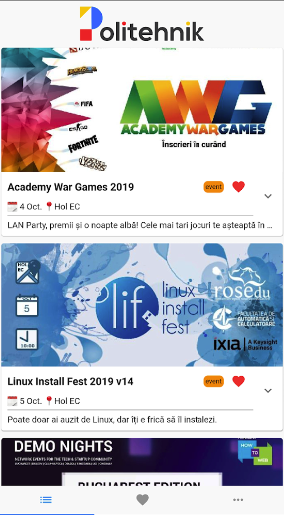
\includegraphics[width=\textwidth]{figures/app/miscellanous/politehnik-1.png}
        \caption{Politehnik-1}
        \label{4:fig:politehnik-1}
    \end{minipage}
    \hfill
    \begin{minipage}[b]{0.25\textwidth}
        \captionsetup{justification=centering}
        
\includegraphics[width=\textwidth]{figures/app/miscellanous/politehnik-2.png}
        \caption{Politehnik-2}
        \label{4:fig:politehnik-2}
    \end{minipage}
    \hfill
    \begin{minipage}[b]{0.24\textwidth}
        \captionsetup{justification=centering}
        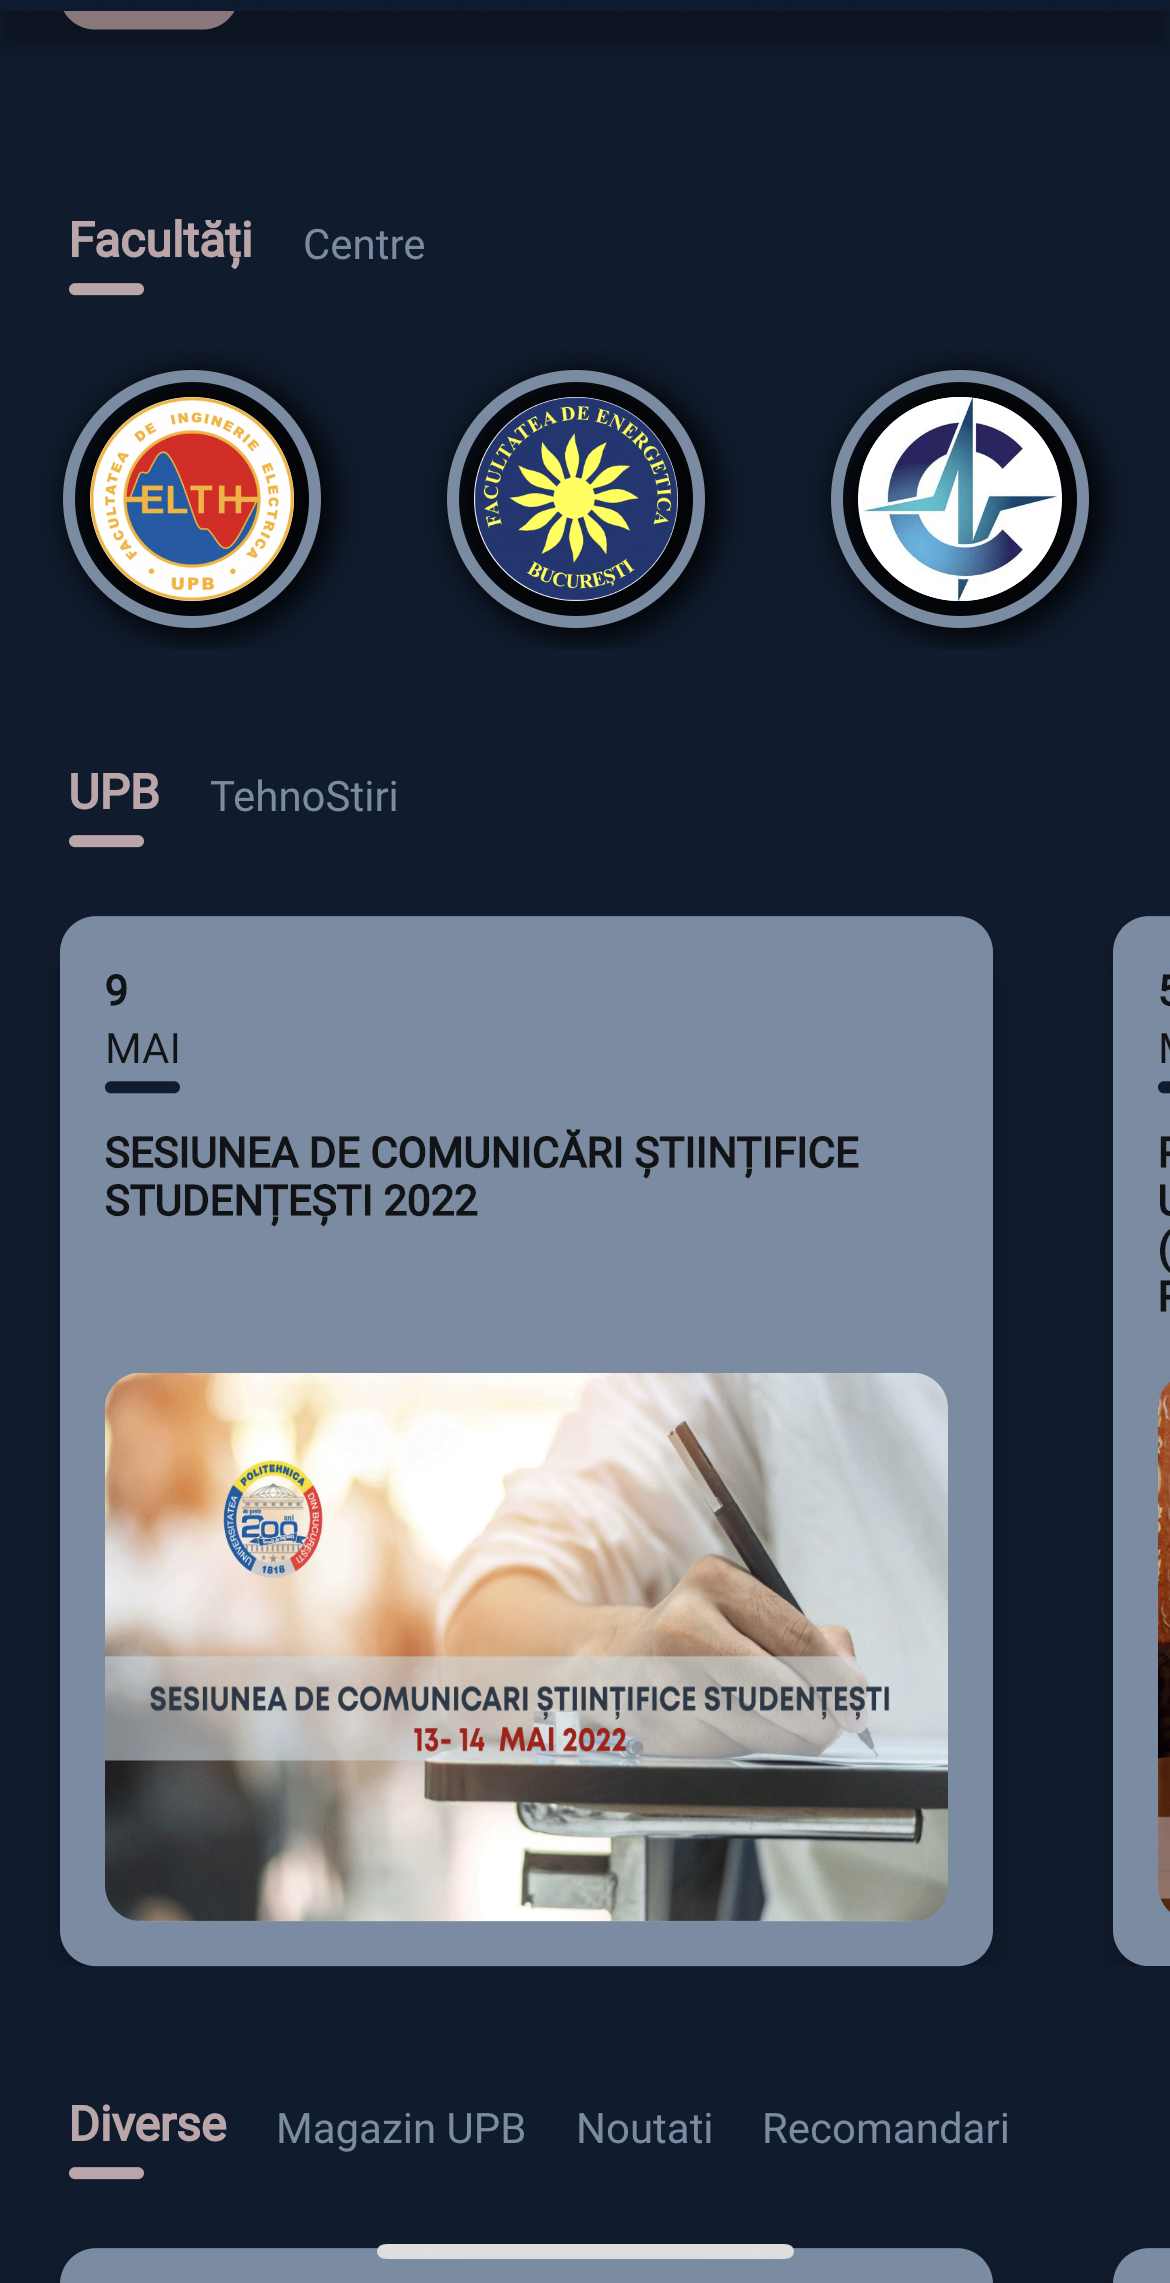
\includegraphics[width=\textwidth]{figures/app/miscellanous/upb-campus-1.png}
        \caption{UPB Campus-1}
        \label{4:fig:upb-campus-1}
    \end{minipage}
    \hfill
    \begin{minipage}[b]{0.23\textwidth}
        \captionsetup{justification=centering}
        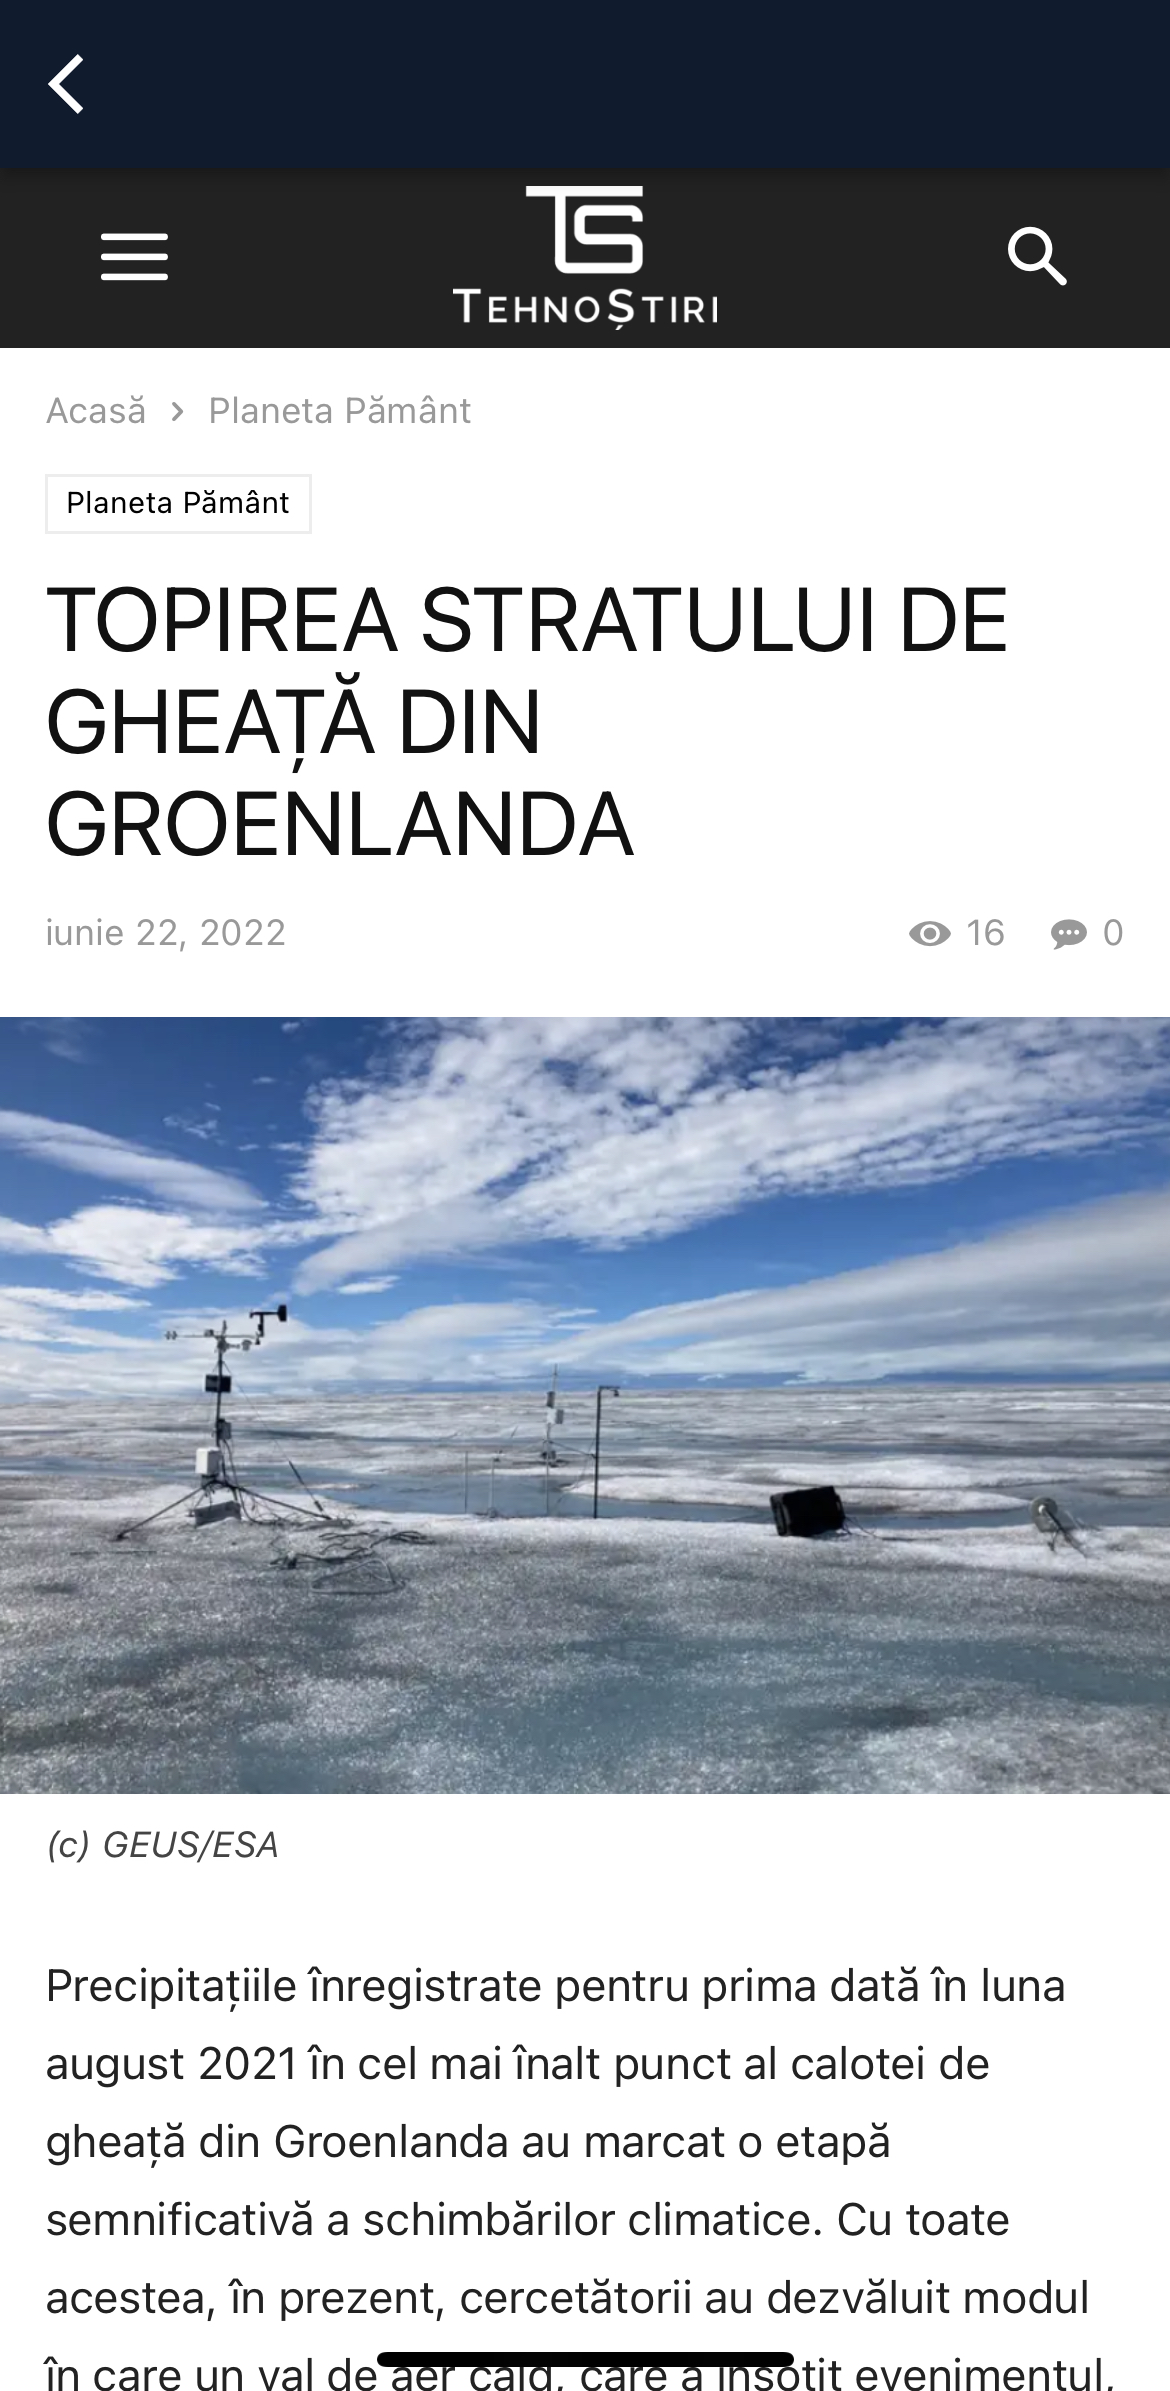
\includegraphics[width=\textwidth]{figures/app/miscellanous/upb-campus-2.png}
        \caption{UPB Campus-2}
        \label{4:fig:upb-campus-2}
    \end{minipage}
\end{figure}

~
On the other hand, \textbf{UPB Campus} is currently maintained by the UPB student \textbf{Diana Scurtu} and is developed using the Flutter framework. The app is available on both Android and iOS, and currently, it displays news from the university website\footnote{https://upb.ro/} and other technical blogs. When discussing with the developer, they revealed that they have the news scraped using HTML scrapers and centralized in a local database. While there is a degree of automation, the information sources are limited, and the news items are more or less in the official category and targeted at the university level.